\documentclass[10pt]{beamer}

\usetheme{CambridgeUS}
\usepackage[english, russian]{babel}
\usepackage[utf8]{inputenc}
\usepackage{caption}
\usepackage{etoolbox}
\usepackage{multicol}
\usepackage{listings}
\usepackage{color}

\definecolor{mygreen}{rgb}{0,0.6,0}
\lstset{
  basicstyle=\ttfamily\footnotesize,        % the size of the fonts that are used for the code
  breaklines=true,                 % automatic line breaking only at whitespace
  captionpos=b,                    % sets the caption-position to bottom
  commentstyle=\color{mygreen},    % comment style
  keywordstyle=\color{blue},       % keyword style
  stringstyle=\color{red},     % string literal style
  showstringspaces=false,
  morekeywords={include, printf},
  texcl=true     %<---- added
}

\title[\href{https://goo.gl/NRgp8K}{https://goo.gl/NRgp8K} (Term 3)]{Ахо-Корасик}
\author[Гусев Илья]{Гусев Илья}
\institute[МФТИ] 
{Московский физико-технический институт\\*}
\date{Москва, 2018}
\subject{Computer Science}

\begin{document}

\begin{frame}
  \titlepage
\end{frame}

\begin{frame}{Содержание}
\tableofcontents
\end{frame}

\section{Алгоритм}
\subsection{Задача}
\begin{frame}[fragile]{Задача}
Дан набор строк $T_0, T_1, ... T_m$, которые мы назовём шаблонами и строка S. Нужно найти все вхождения $T_i$  в S.  
\end{frame}

\subsection{Бор}
\begin{frame}[fragile]{Бор}{Структура данных}
\begin{multicols}{2}
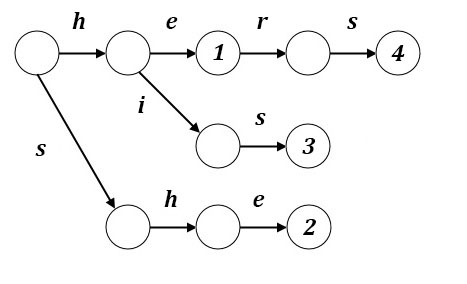
\includegraphics[width=6cm, height=3.7cm]{Term_3/Source/Pictures/bor.jpg}
\vfill\eject
Шаблоны:
\begin{itemize}
    \item hers\\
    \item his\\
    \item she\\
    \item he\\
\end{itemize}
\end{multicols}
\end{frame}

\begin{frame}[fragile]{Бор}{Варианты хранения}
\begin{enumerate}
    \item Нода: array ссылок
    \item Нода: map/unordered\_map ссылок
\end{enumerate}
\end{frame}

\subsection{Алгоритм}
\begin{frame}[fragile]{Суффиксные ссылки}
$parent(u)$ - родитель u \\
$\pi(u) = \delta(\pi(parent(u)),c)$ - суффиксная ссылка\\
$\delta(u,c) = v$, если из u есть переход в v по c\\
$\delta(u,c) = root$, если u - корень и из него нет перехода по c\\
$\delta(u,c) = \delta(\pi(u), c)$, иначе\\
\end{frame}

\begin{frame}[fragile]{Сжатые суффиксные ссылки}
$up(u) = \pi(u)$, если $\pi(u)$ - терминальная вершина\\
$up(u) = \emptyset$, если $\pi(u)$ - корень\\
$up(u) = up(\pi(u))$, иначе\\
\end{frame}

\begin{frame}[fragile]{Автомат}
\begin{multicols}{2}
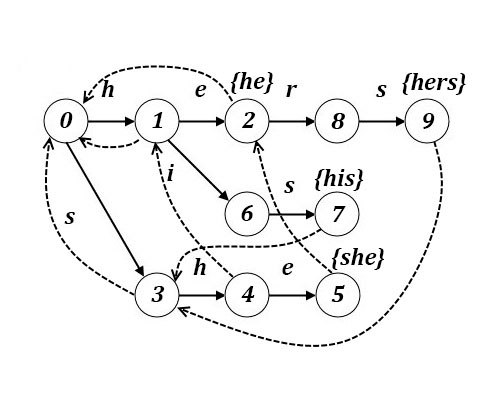
\includegraphics[width=6cm, height=5cm]{Term_3/Source/Pictures/aho.jpg}
\vfill\eject
Шаблоны:
\begin{itemize}
    \item hers\\
    \item his\\
    \item she\\
    \item he\\
\end{itemize}

\end{multicols}
\end{frame}

\section{Задачи}

\subsection{Вопросики}
\begin{frame}[fragile]{Вопросики}
Поиск шаблона ab??ceee?dg. Знаки вопроса - любой символ (не путайте с regex ?).
\end{frame}

\subsection{Вирусы}
\begin{frame}[fragile]{Вирусы}
Есть вирусы - конечные пути $V_1,...,V_k$.\\
Существует ли бесконечно много 'здоровых' файлов?
\end{frame}

\appendix
\section<presentation>*{\appendixname}
\subsection<presentation>*{Useful links}

\begin{frame}[allowframebreaks]
  \frametitle<presentation>{Полезные ссылки}
    
  \begin{thebibliography}{10}
{
  \beamertemplatebookbibitems
  % Start with overview books.

  
  \bibitem{neerc}
  \texttt{Викиконспекты: Ахо-Корасик}
  \newblock \href{https://bit.ly/2Qq3cod}{\texttt{http://neerc.ifmo.ru/wiki/index.php?title=Алгоритм\_Ахо-Корасик}}
  
  \bibitem{e-maxx}
  \texttt{E-maxx: Ахо-Корасик}
  \newblock \href{http://www.e-maxx-ru.1gb.ru/algo/aho_corasick}{\texttt{http://www.e-maxx-ru.1gb.ru/algo/aho\_corasick}}
  
}
    
  \end{thebibliography}
\end{frame}

\end{document}


